\section{Dataset}
We gather the data from Huawei garbage classification challenge task and Kaggle garbage classification competition.
Source datasets:
\begin{enumerate}
    \item Huawei: \\
          Size in total: 14683\\
          Number of classes: 40\\
          Source: \href{https://developer.huaweicloud.com/hero/forum.php?mod=viewthread&tid=24106}{[Published page]}
          or the direct download \href{https://modelarts-competitions.obs.cn-north-1.myhuaweicloud.com/garbage_classify/dataset/garbage_classify_v2.zip}{[link]} \\
          We use Huawei dataset as our base dataset.
    \item Kaggle: \\
          Size in total: 2467\\
          Size included: 2371\\
          Source: \href{https://www.kaggle.com/asdasdasasdas/garbage-classification}{[Published page]}\\
          The Kaggle dataset oririnally contains 5 classes (cardboard (393), glass (491), metal (400), paper(584), plastic (472) and trash (127)). 
          We manually classify the Kaggle images with the labels in Huawei dataset. For those can not be directly classified, 
          we add extra labels if the amount of images is relative large and exclude others with few samples.
\end{enumerate}
%
The sorted combined dataset:\\
Size in total: 17054\\
Number of classes: 42 (40 classes from Huawei dataset and 2 classes from Kaggle dataset)\\
Size of training set: 15522\\
Size of test set: 1532\\
Besides the Kaggle dataset, we have considered the images from ImageNet dataset. However, the images from ImageNet are all with 
messy backgrounds, which is quite different from Huawei and Kaggle data, thus we did not add these images.
\begin{figure}[ht]
    \centering
    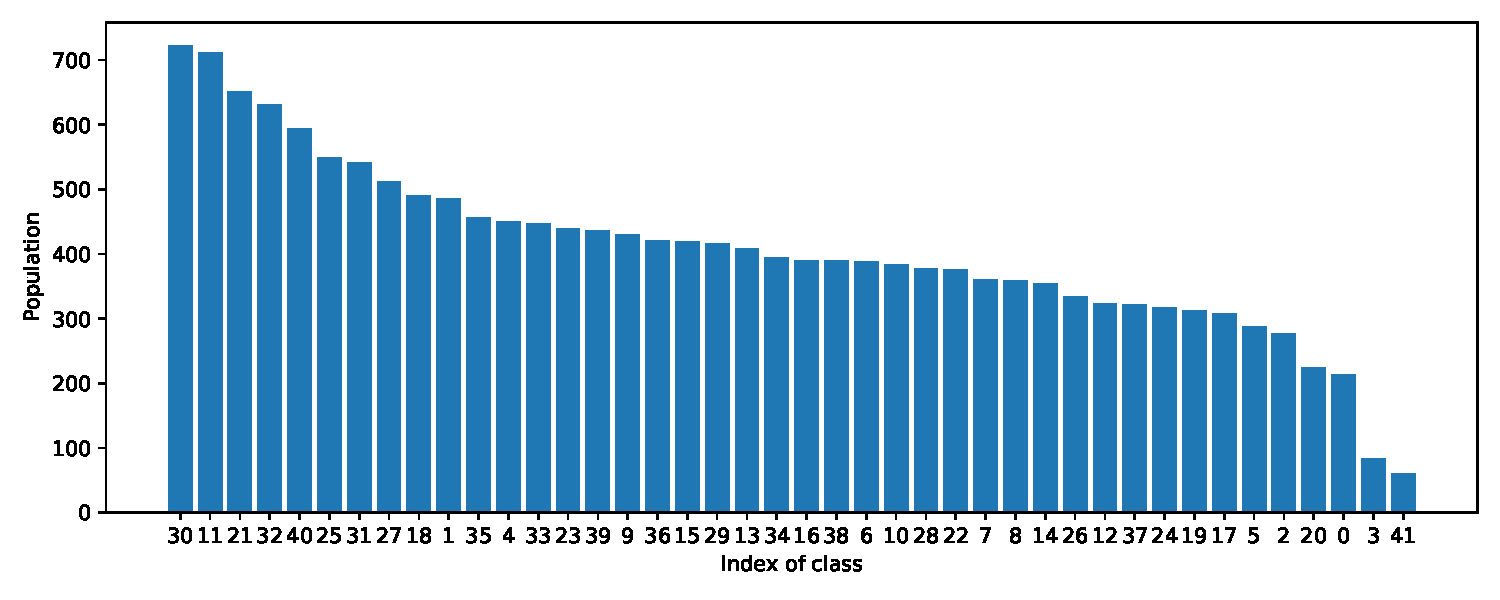
\includegraphics[width=\linewidth]{figs/dist_dataset.pdf}
    \caption{The population of all classes in our combined dataset.}
\end{figure}